\documentclass{article}
\usepackage[margin=1in]{geometry}
\usepackage{fancyvrb}
\usepackage{multicol}
\usepackage{hyperref}
\usepackage{amsmath}
\usepackage{amsfonts}

\usepackage[listings]{tcolorbox}

\definecolor{codegreen}{rgb}{0,0.6,0}
\definecolor{codegray}{rgb}{0.5,0.5,0.5}
\definecolor{codepurple}{rgb}{0.58,0,0.82}
\definecolor{backcolour}{rgb}{0.95,0.95,0.92}

\lstdefinestyle{mystyle}{
    language=Python,
    backgroundcolor=\color{backcolour},   
    commentstyle=\color{codegreen},
    keywordstyle=\color{magenta},
    numberstyle=\tiny\color{codegray},
    stringstyle=\color{codepurple},
    basicstyle=\ttfamily\footnotesize,
    breakatwhitespace=false,         
    breaklines=true,                 
    captionpos=b,                    
    keepspaces=true,                 
    numbers=left,                    
    numbersep=5pt,                  
    showspaces=false,                
    showstringspaces=false,
    showtabs=false,                  
    tabsize=2,
    escapechar=|,
    frame=single
}

\lstset{style=mystyle}

%\usepackage[T1]{fontenc}
\usepackage{tikz}
\usetikzlibrary{arrows.meta,
                calc, chains,
                decorations.pathreplacing,
                calligraphy,
                positioning,
                quotes,
                shapes}
                
\newcommand{\showfig}[2]{
\noindent\includegraphics[width=\textwidth]{#1}
\centerline{#1}
}
\newcommand{\bi}{\begin{itemize}}
\newcommand{\li}{\item}
\newcommand{\ei}{\end{itemize}}

\title{Infix Calculator}
\author{CSCI 112, Lab 4}
\date{}

\begin{document}
\sloppy

\maketitle

\begin{description} 
\item[File names:]  Names of files, functions, and variables, 
when specified,
must be EXACTLY as specified.  This includes simple mistakes such
as capitalization.

\item[Individual work:]  All work must be your own.  Do not share
code with anyone other than the instructor and teaching assistants.
This includes looking over shoulders at screens with the code open.
You may discuss ideas, algorithms, approaches, {\em etc.} with
other students but NEVER actual code.  Do not use code
written by anyone else, in the class or from the internet.

\item[Documentation:] Each file should begin with a docstring
that includes your name, the class number and name, the lab
number, and  
a short description of the lab, as well as documentation pertinent
to that particular file.

\item[Addition and subtraction standard algorithm:]  You should be
familiar with the standard algorithms for addition and subtractin,
at least in base 10.  If you are not familiar with other number bases,
review them quickly here: \url{https://www.mathsisfun.com/numbers/bases.html}.

The standard subtraction and addition algorithms work fine in any
base.  You just have to remember that if you are in base 16, say,
and you ``borrow one'' from the next column, you are borrowing 16,
not 10.  Likewise, if you carry one to the next column, you are
carrying 16, not 10.  Here are some worked examples to get
the hang of things:

Base 10 examples:\hfill
\begin{tabular}{rrrrr}
  &3 &9 &1 &5\\
$+$ &1 &2 &4 &5\\
\hline
  &5 &1 &6 &0\\
\end{tabular}\hfill
\begin{tabular}{rrrrr}
  &3 &9 &1 &5\\
$-$ &1 &2 &4 &5\\
\hline
  &2 &6 &7 &0\\
\end{tabular}

Base 8 examples:\hfill
\begin{tabular}{rrrrrr}
  &  &7 &5 &1 &3\\
$+$ &  &2 &3 &3 &5\\
\hline
  &1 &2 &0 &5 &0\\
\end{tabular}\hfill
\begin{tabular}{rrrrr}
  &7 &5 &1 &3\\
$-$ &2 &3 &3 &5\\
\hline
  &5 &1 &5 &6\\
\end{tabular}

Base 16 examples:\hfill
\begin{tabular}{rrrrr}
  &  &15 &4 &11\\
$+$ &  &4 &13 &13\\
\hline
  &1 &4 &2 &8\\
\end{tabular}\hfill
\begin{tabular}{rrrr}
  &15 &4 &11\\
$-$ &4 &13 &13\\
\hline
  &10 &6 &14\\
\end{tabular}

If you want more examples, just run my program {\tt arithmetic.py}
and paste the output into a new project on \url{https://www.overleaf.com}.

You can get easy base 8 and base 16 examples from python:
\begin{lstlisting}
>>> hex(0xaaa + 0x123)
'0xbcd'
>>> oct(0o666 + 0o123)
'0o1011'
\end{lstlisting}




    \begin{figure}[ht]
    \centering
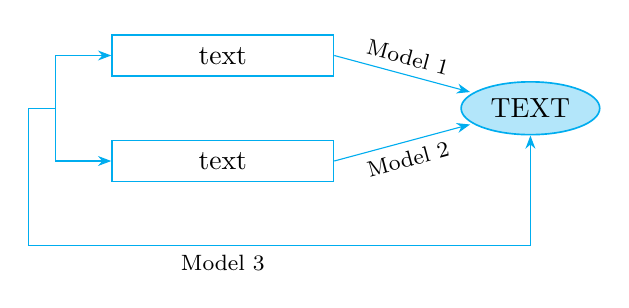
\begin{tikzpicture}[
node distance = 8mm and 16mm,
            > = Stealth,
every path/.append style = {draw=cyan},
every edge quotes/.append style = {font=\footnotesize, sloped},
     E/.style = {ellipse, draw, semithick, fill=cyan!30},
     N/.style = {draw, semithick, minimum width = 8em, inner sep=1ex}
                    ]
\node (a) [N]  {text};
\node (b) [N, below=of a]  {text};
\node (e) [E, right=of {$(a.east)!0.5!(b.east)$}]  {TEXT};
%
\coordinate[below=of b.south] (aux);
\draw[<->]  (a.west) -- ++ (-2em,0) |- (b.west) coordinate[pos=0.25] (ab);
\draw[->]   (ab) -- ++ (-1em,0) 
                 |- (aux) node[below, font=\footnotesize] {Model 3} 
                 -| (e);
\draw[->, shorten >=1pt]   (a.east) to ["Model 1"]     (e);
\draw[->, shorten >=1pt]   (b.east) to ["Model 2" ']   (e);
\end{tikzpicture}
    \end{figure}
    
\end{description}



\end{document}
